\documentclass[12pt]{article}
\usepackage{graphicx}
\usepackage[margin=1in]{geometry}

\begin{document}
\title{Graph Theory \& Surface Reconstruction}
\author{Jenny Zhen}
\date{April 25, 2013}
\maketitle

\begin{abstract}The purpose of this paper is to utilize a technique for recreating models of 3-D objects. This process is referred to as surface reconstruction, which replaces a set of sample points using a faceted geometric model. Concepts of graph theory are used, specifically duals of graphs, n-regular graphs, bridgeless graphs, and matchings.
\end{abstract}

\begin{flushleft}
\section*{Introduction}
The paper will refer to the triangulation of a 3-D surface given in the figure below.

\begin{center}
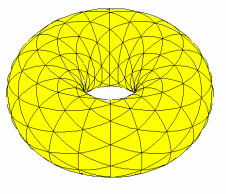
\includegraphics[scale=1]{images/torus1.png}\\
Figure 1: A torus.
\end{center}

The figure resembles a torus, which is created by revolving a circle along a line made by another circle. Divisions of polygonal faces that form the torus produces triangular faces throughout the torus.

\subsection*{Dual Graph}
By definition, the planar dual of any planar graph, G, can be constructed by placing a vertex in each region of G and then adding edges between regions that share a border. The planar dual is denoted as D(G).

\medskip
If a dual of the torus is to be constructed, the same procedure to create the dual of a planar graph will be used. A point will be placed in each of the triangular faces, then lines between pairs of vertices would be placed, if and only if, the corresponding faces share a common side. The dual of the torus, G, is constructed below.

\begin{center}
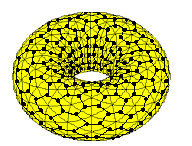
\includegraphics[scale=1.25]{images/torus2.png}\\
Figure 2: Dual of a torus, G.
\end{center}

As shown in the figure, the triangular faces of the original torus are hexagonal faces in the dual of the torus.

\subsection*{n-regular Graph}
A graph is considered n-regular if every vertex in the graph is incident to exactly n edges.

\medskip
The dual of the torus is a 3-regular graph. According to the definition, that would mean that every vertex in the dual of the torus, G, is incident to exactly 3 edges. The graph of the dual is a 3-regular because each face in the original graph is a complete graph, $K_3$, in which each vertex is connected to all the other vertices. A $K_3$ graph consists of 3 vertices that all have degree 2. The dual of a $K_3$ is just one vertex inside the cycle and one vertex on the outside of the cycle, which represents the infinite region. Each edge in $K_3$ has an edge in the dual graph crossing the edge to connect those two vertices, as shown below.

\begin{center}
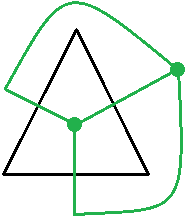
\includegraphics[scale=1]{images/k3dual.png}\\
Figure 2: Dual of a complete graph, $K_3$.
\end{center}

\medskip
By taking the dual of groups of $K_3$, a similar concept is used to connect the vertices for each region, excluding the infinite region. As a result of the three edges in each $K_3$, each vertex representing one region has three incident edges in the planar dual graph of each $K_3$. Thus, the dual of the torus is a 3-regular graph.

\subsection*{Bridgeless Graph}

\end{flushleft}
\end{document}